\documentclass[11pt,a4paper]{article}
\usepackage[utf8]{inputenc}
\usepackage[T1]{fontenc}
\usepackage[margin=2.5cm]{geometry}
\usepackage{amsmath,amssymb,bm}
\usepackage{graphicx}
\usepackage{float}
\usepackage[hidelinks]{hyperref}
\usepackage{booktabs}

\newcommand{\mat}[1]{\mathbf{#1}}
\newcommand{\vc}[1]{\bm{#1}}
\newcommand{\hkl}[1]{\left(#1\right)}
\newcommand{\uvw}[1]{\left[#1\right]}
\newcommand{\trace}{\operatorname{tr}}

\title{Estimation of Habit Planes from Interface Traces in 2D EBSD Maps\\[4pt]
\large Method description of the \texttt{EbsdHPAnalyzer} class in \texttt{ebsdlib}}
\author{}
\date{\today}

\begin{document}
\maketitle

\begin{abstract}
This report describes the trace-analysis method implemented in the \texttt{EbsdHPAnalyzer} class of \texttt{ebsdlib} for estimating habit (interface) planes between a parent phase (austenite) and lamellar child phase (martensite) from two-dimensional EBSD orientation maps. A single planar section only reveals the \emph{trace} of an interface plane, i.e.\ its intersection line with the scan surface, leaving a one-parameter family of crystallographic planes compatible with the observation. The method resolves this ambiguity by (i) generating all low-index plane candidates that contain the measured trace, independently in both phases, (ii) requiring the candidate plane normals of the two phases to coincide in the sample reference frame, (iii) requiring matching in-plane lattice directions in both phases, and (iv) checking consistency with the lattice correspondence of the martensite variant identified from the experimental orientation relationship. Candidates are ranked by a combined score favoring low Miller indices, small angular misalignments and a large number of corresponding in-plane directions.
\end{abstract}

\section{Input data and notation}

\begin{figure}[H]
\centering
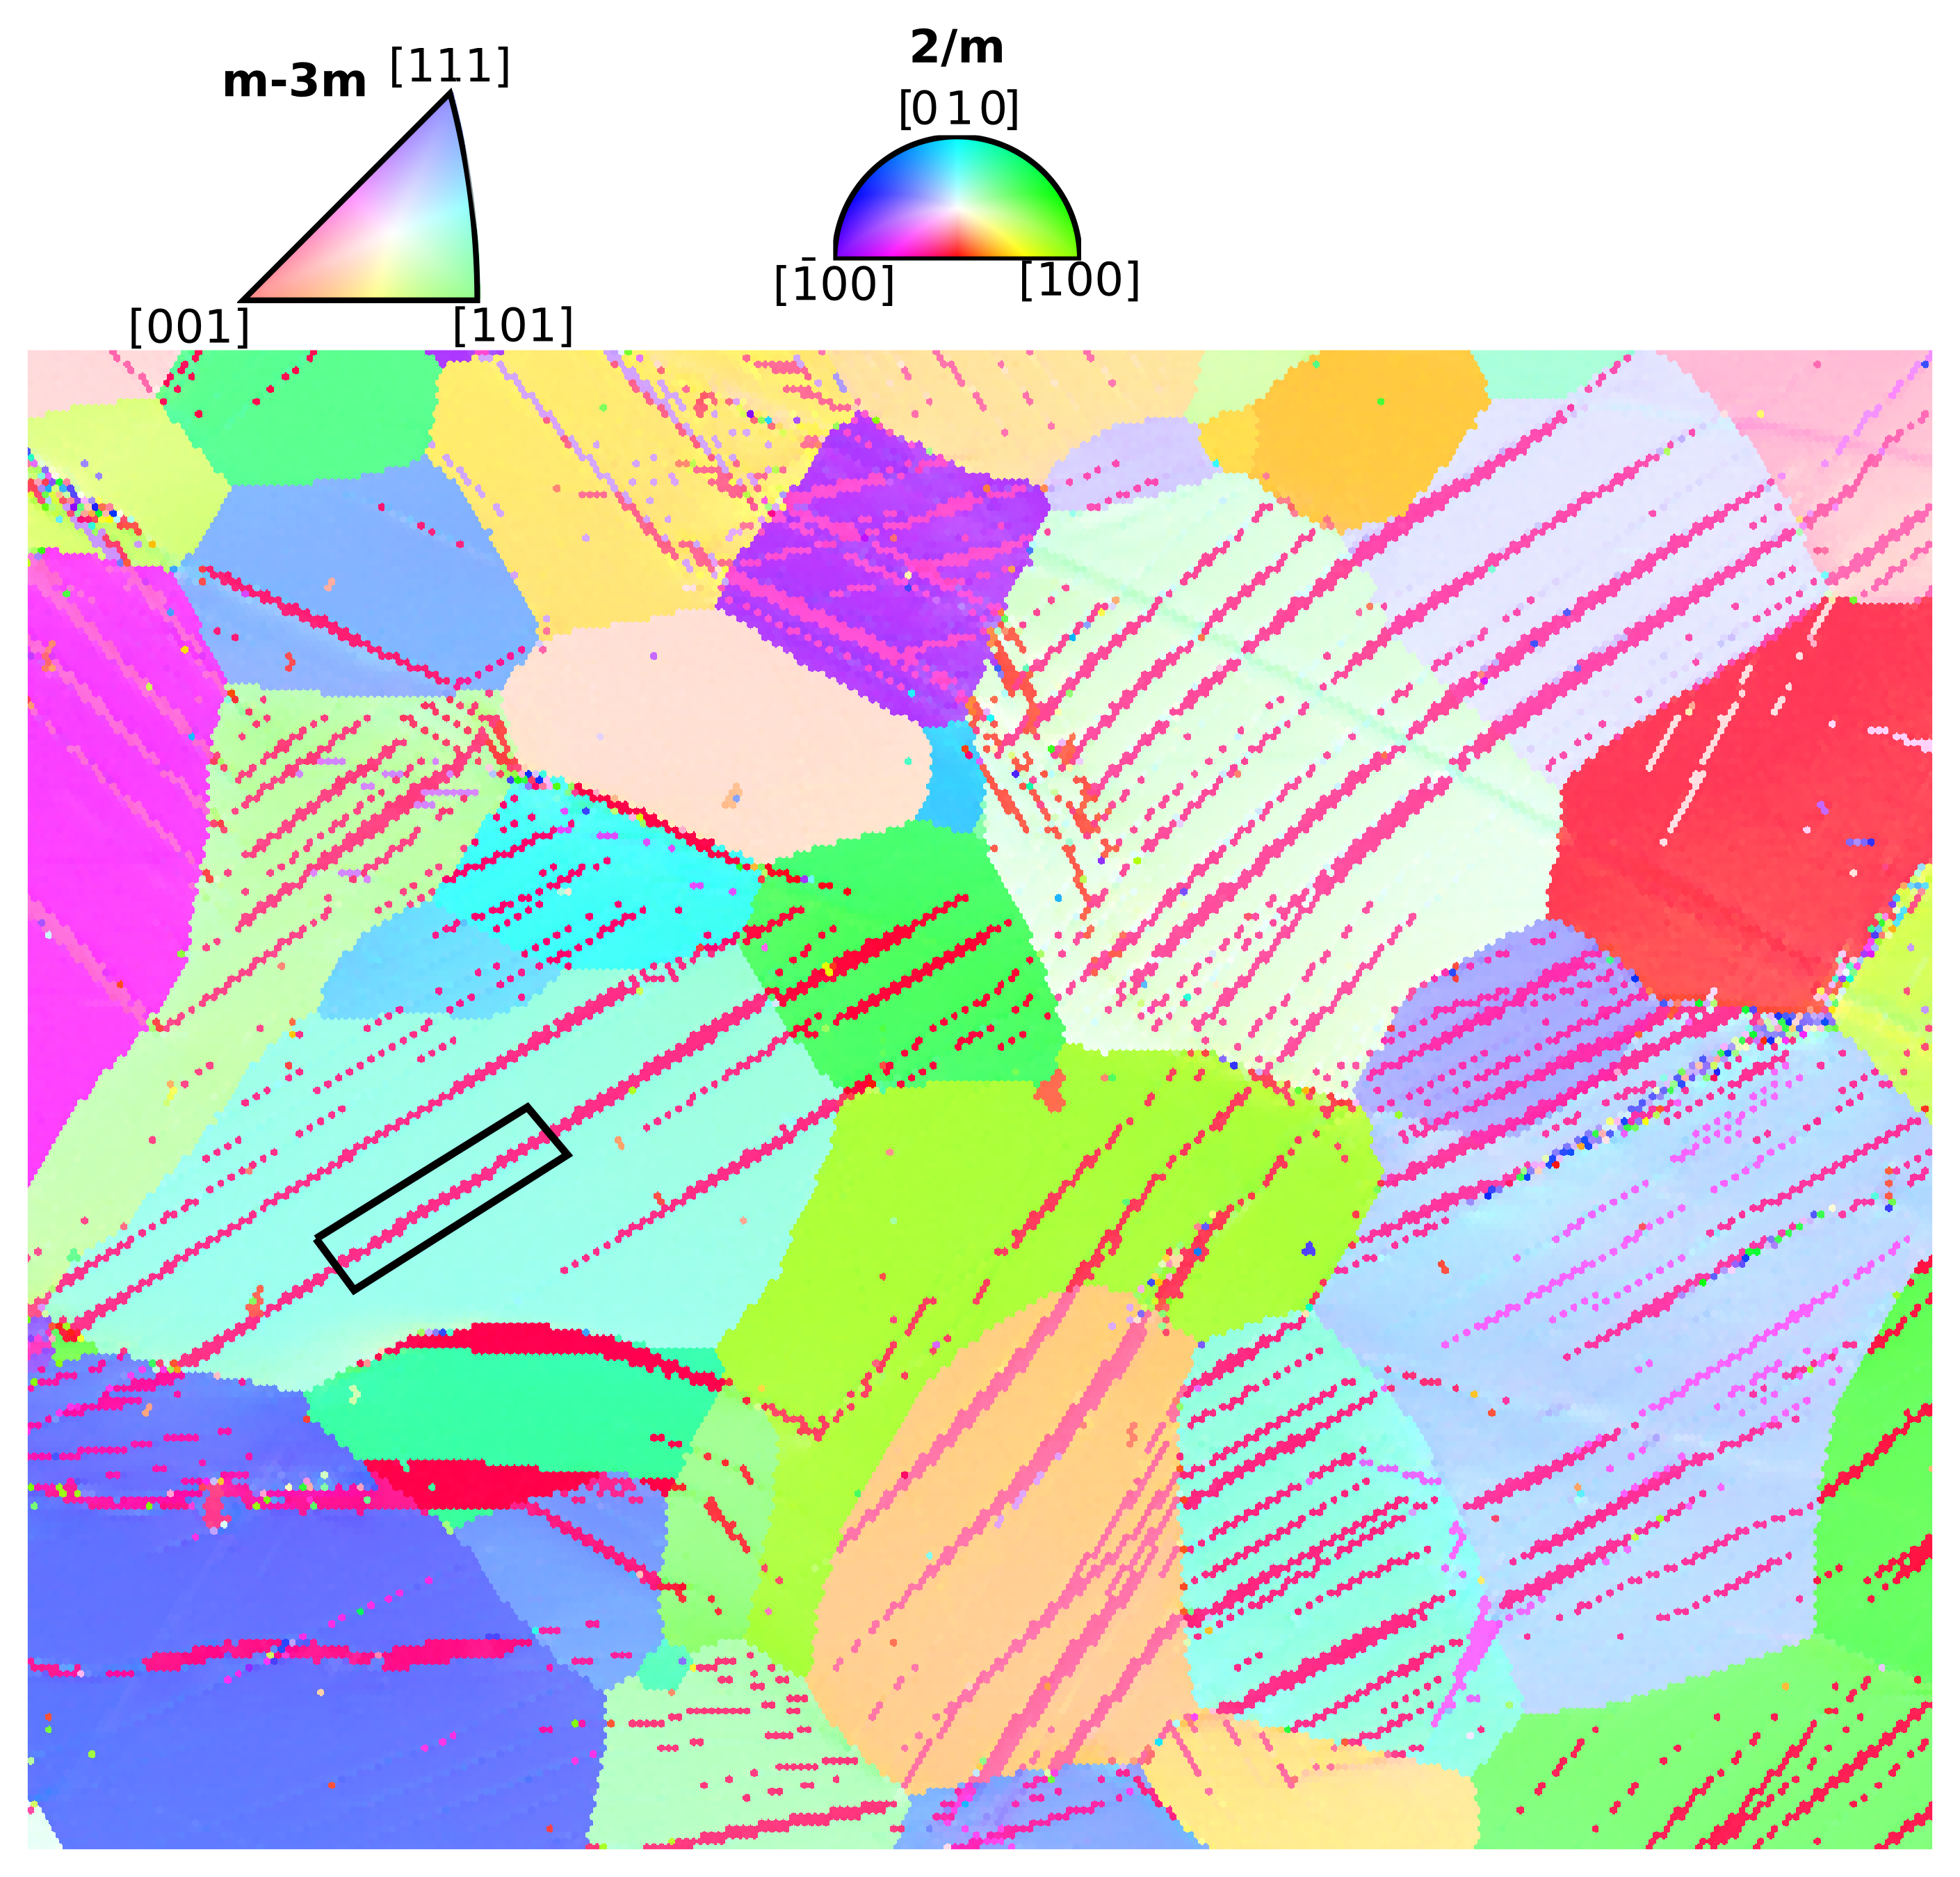
\includegraphics[width=0.78\linewidth]{./figs/figA.png}
\caption{Selection of a region of interest (ROI) on the EBSD orientation map. Austenite grains are coloured by their inverse pole figure (cubic $m\bar{3}m$ key) and the lamellar martensite by the monoclinic $2/m$ key; the lamellae appear as fine parallel traces inside the parent grains. A single lamella (black rectangle) together with its two interface sides defines the ROI on which the habit-plane analysis is performed.}
\label{fig:roi}
\end{figure}

The analysis operates on the output of the clustering and boundary-analysis pipeline of \texttt{ebsdlib}. The method \texttt{BoundaryResult.get\_parent\_child\_hierarchy\_with\_boundaries} provides, for every parent cluster of the austenite phase, the set of enclosed or touching child clusters of the martensite phase. Children with a sufficiently large aspect ratio (default $\mathrm{AR}\geq 2.5$, determined by PCA of the cluster pixel cloud) are flagged as \emph{lamellar} and their interfaces are split into two semi-regions of interest (semi-ROIs), one for each long side of the lamella. For each semi-ROI the hierarchy stores the boundary pixel coordinates $(X_i,Y_i)$ on the parent side and on the child side, together with the symmetry-reduced per-pixel orientation matrices and their iteratively computed averages, denoted below by $\mat{G}^{\mathrm{A}}$ (austenite) and $\mat{G}^{\mathrm{M}}$ (martensite). Throughout this report $\mat{G}^{\varphi}$ is the average sample-to-crystal transformation matrix of phase $\varphi$ (\texttt{G2Cryst\_red\_avg}), mapping sample directions into the crystal coordinate system; the transposed matrix $\mat{G}^{\varphi\,\mathsf{T}}$ (\texttt{G2Sampl\_red\_avg}) maps crystal vectors to the sample frame.

For each phase $\varphi$ the crystal lattice is described by its structure matrix $\mat{L}^{\varphi}$ (columns are the lattice basis vectors in the Cartesian crystal frame) and the reciprocal structure matrix $\mat{L}_{r}^{\varphi}$ (columns are the reciprocal basis vectors), so that a plane with Miller indices $\vc{h}^{\varphi}=(h\,k\,l)^{\mathsf T}$ has the Cartesian normal
\begin{equation}
\vc{\nu}^{\varphi}(\vc h^{\varphi})=\frac{\mat{L}_{r}^{\varphi}\,\vc h^{\varphi}}{\lVert \mat{L}_{r}^{\varphi}\,\vc h^{\varphi}\rVert},
\label{eq:nu}
\end{equation}
and a direction $\vc{u}^{\varphi}=[u\,v\,w]^{\mathsf T}$ has the Cartesian unit vector $\mat{L}^{\varphi}\vc u^{\varphi}/\lVert\mat{L}^{\varphi}\vc u^{\varphi}\rVert$. The inverse matrices $(\mat{L}^{\varphi})^{-1}$ and $(\mat{L}_{r}^{\varphi})^{-1}$ are used to convert Cartesian vectors back to (fractional) Miller indices, which are subsequently rounded to the smallest integer triplet.

The martensitic transformation data of the material (NiTi in the present implementation) enter through the rotational parts $\mat{T}^{(v)}_{\mathrm{AM}}$ of the theoretical orientation relationship for each lattice-correspondence variant $v$, the deformation gradients $\mat{F}^{(v)}_{\mathrm{AM}}$, and the integer lattice-correspondence matrices for planes, $\mat{C}_p^{(v)}$, and for directions, $\mat{C}_d^{(v)}$, which map austenite Miller indices to martensite Miller indices of the same lattice plane or direction.

\section{Interface trace from the boundary geometry}

The boundary pixel coordinates of the parent and child side of a semi-ROI are pooled into a single point set $\{(X_i,Y_i)\}$ and a straight line is fitted by linear least squares, $y = k\,x + q$ (\texttt{np.polyfit} of degree one in \texttt{getInterface}). The unit trace vector and the in-plane unit normal of the trace in the sample (scan) frame are
\begin{equation}
\vc t^{\,s}=\frac{1}{\sqrt{1+k^{2}}}\begin{pmatrix}1\\ k\\ 0\end{pmatrix},
\qquad
\vc m^{\,s}=\frac{1}{\sqrt{1+1/k^{2}}}\begin{pmatrix}1\\ -1/k\\ 0\end{pmatrix},
\label{eq:trace}
\end{equation}
where the third coordinate is the scan normal. Both vectors are transformed into the crystal frame of each phase,
\begin{equation}
\vc t^{\,\varphi}=\mat{G}^{\varphi}\,\mat P\,\vc t^{\,s},
\qquad
\vc m^{\,\varphi}=\mat{G}^{\varphi}\,\mat P\,\vc m^{\,s},
\qquad
\mat P=\begin{pmatrix}0&1&0\\ 1&0&0\\ 0&0&1\end{pmatrix},
\label{eq:crystal_trace}
\end{equation}
where the permutation matrix $\mat P$ (\texttt{CrystalRef2Spatial}) accounts for the convention difference between the EBSD scan axes and the crystal reference used by the orientation matrices.

The key geometric fact exploited by the method is that the true habit plane must \emph{contain} the trace: its normal $\vc n$ satisfies $\vc n\perp\vc t$. A single section therefore constrains the normal only to the plane perpendicular to $\vc t$, leaving one free rotation angle.

\section{Generation of candidate plane normals}

The one-parameter family of admissible normals is sampled in \texttt{getNormals} by rotating the in-plane trace normal about the trace axis,
\begin{equation}
\vc n^{\varphi}(\alpha)=\mat R(\vc t^{\,\varphi},\alpha)\,\vc m^{\,\varphi},
\qquad \alpha \in [0^\circ,180^\circ]
\label{eq:family}
\end{equation}
with a step of $0.5^\circ$, where $\mat R(\vc a,\alpha)$ denotes the rotation by angle $\alpha$ about axis $\vc a$. Each sampled normal is converted to approximate Miller indices through
\begin{equation}
\vc h^{\varphi}(\alpha)=\operatorname{round}\!\Big[\operatorname{red}\big((\mat{L}_{r}^{\varphi})^{-1}\,\vc n^{\varphi}(\alpha)\big)\Big],
\label{eq:miller}
\end{equation}
where $\operatorname{red}(\cdot)$ rescales the fractional triplet to the smallest near-integer representation (\texttt{vector2millerround}; if the result exceeds the index limit, an alternative normalization is attempted). The rounding generally moves the plane slightly off the sampled direction, so the exact normal $\vc \nu^{\varphi}(\vc h^{\varphi})$ of the rounded plane, Eq.~\eqref{eq:nu}, is recomputed and the candidate is accepted only if it still contains the trace within tolerance and remains low-index:
\begin{equation}
\big|\theta^{\varphi}(\vc h^{\varphi})-90^\circ\big|\le \delta_{90},
\qquad
\theta^{\varphi}(\vc h^{\varphi})=\arccos\big|\vc\nu^{\varphi}(\vc h^{\varphi})\cdot\vc t^{\,\varphi}\big|,
\qquad
\max_i |h^{\varphi}_i|\le h_{\max},
\label{eq:accept}
\end{equation}
with defaults $\delta_{90}=4^\circ$ (\texttt{maxdevfrom90deg}) and $h_{\max}=4$ (\texttt{maxmillerindex}). The superscript $\varphi\in\{\mathrm A,\mathrm M\}$ indicates that the test is carried out independently in each phase, with the candidate normal and the trace both expressed in that phase's crystal frame. Antiparallel duplicates $\pm\vc h^{\varphi}$ are merged. For every accepted candidate the code stores the Miller indices, the family $\{hkl\}$ they belong to (from a precomputed symmetry-expanded table generated by \texttt{generate\_hkls}), the exact Cartesian normal in the crystal frame and its image in the sample frame, $\vc \nu^{\varphi,s}=\mat{G}^{\varphi\,\mathsf T}\vc\nu^{\varphi}$, and the trace-containment angle $\theta^{\varphi}$.

\begin{figure}[H]
\centering
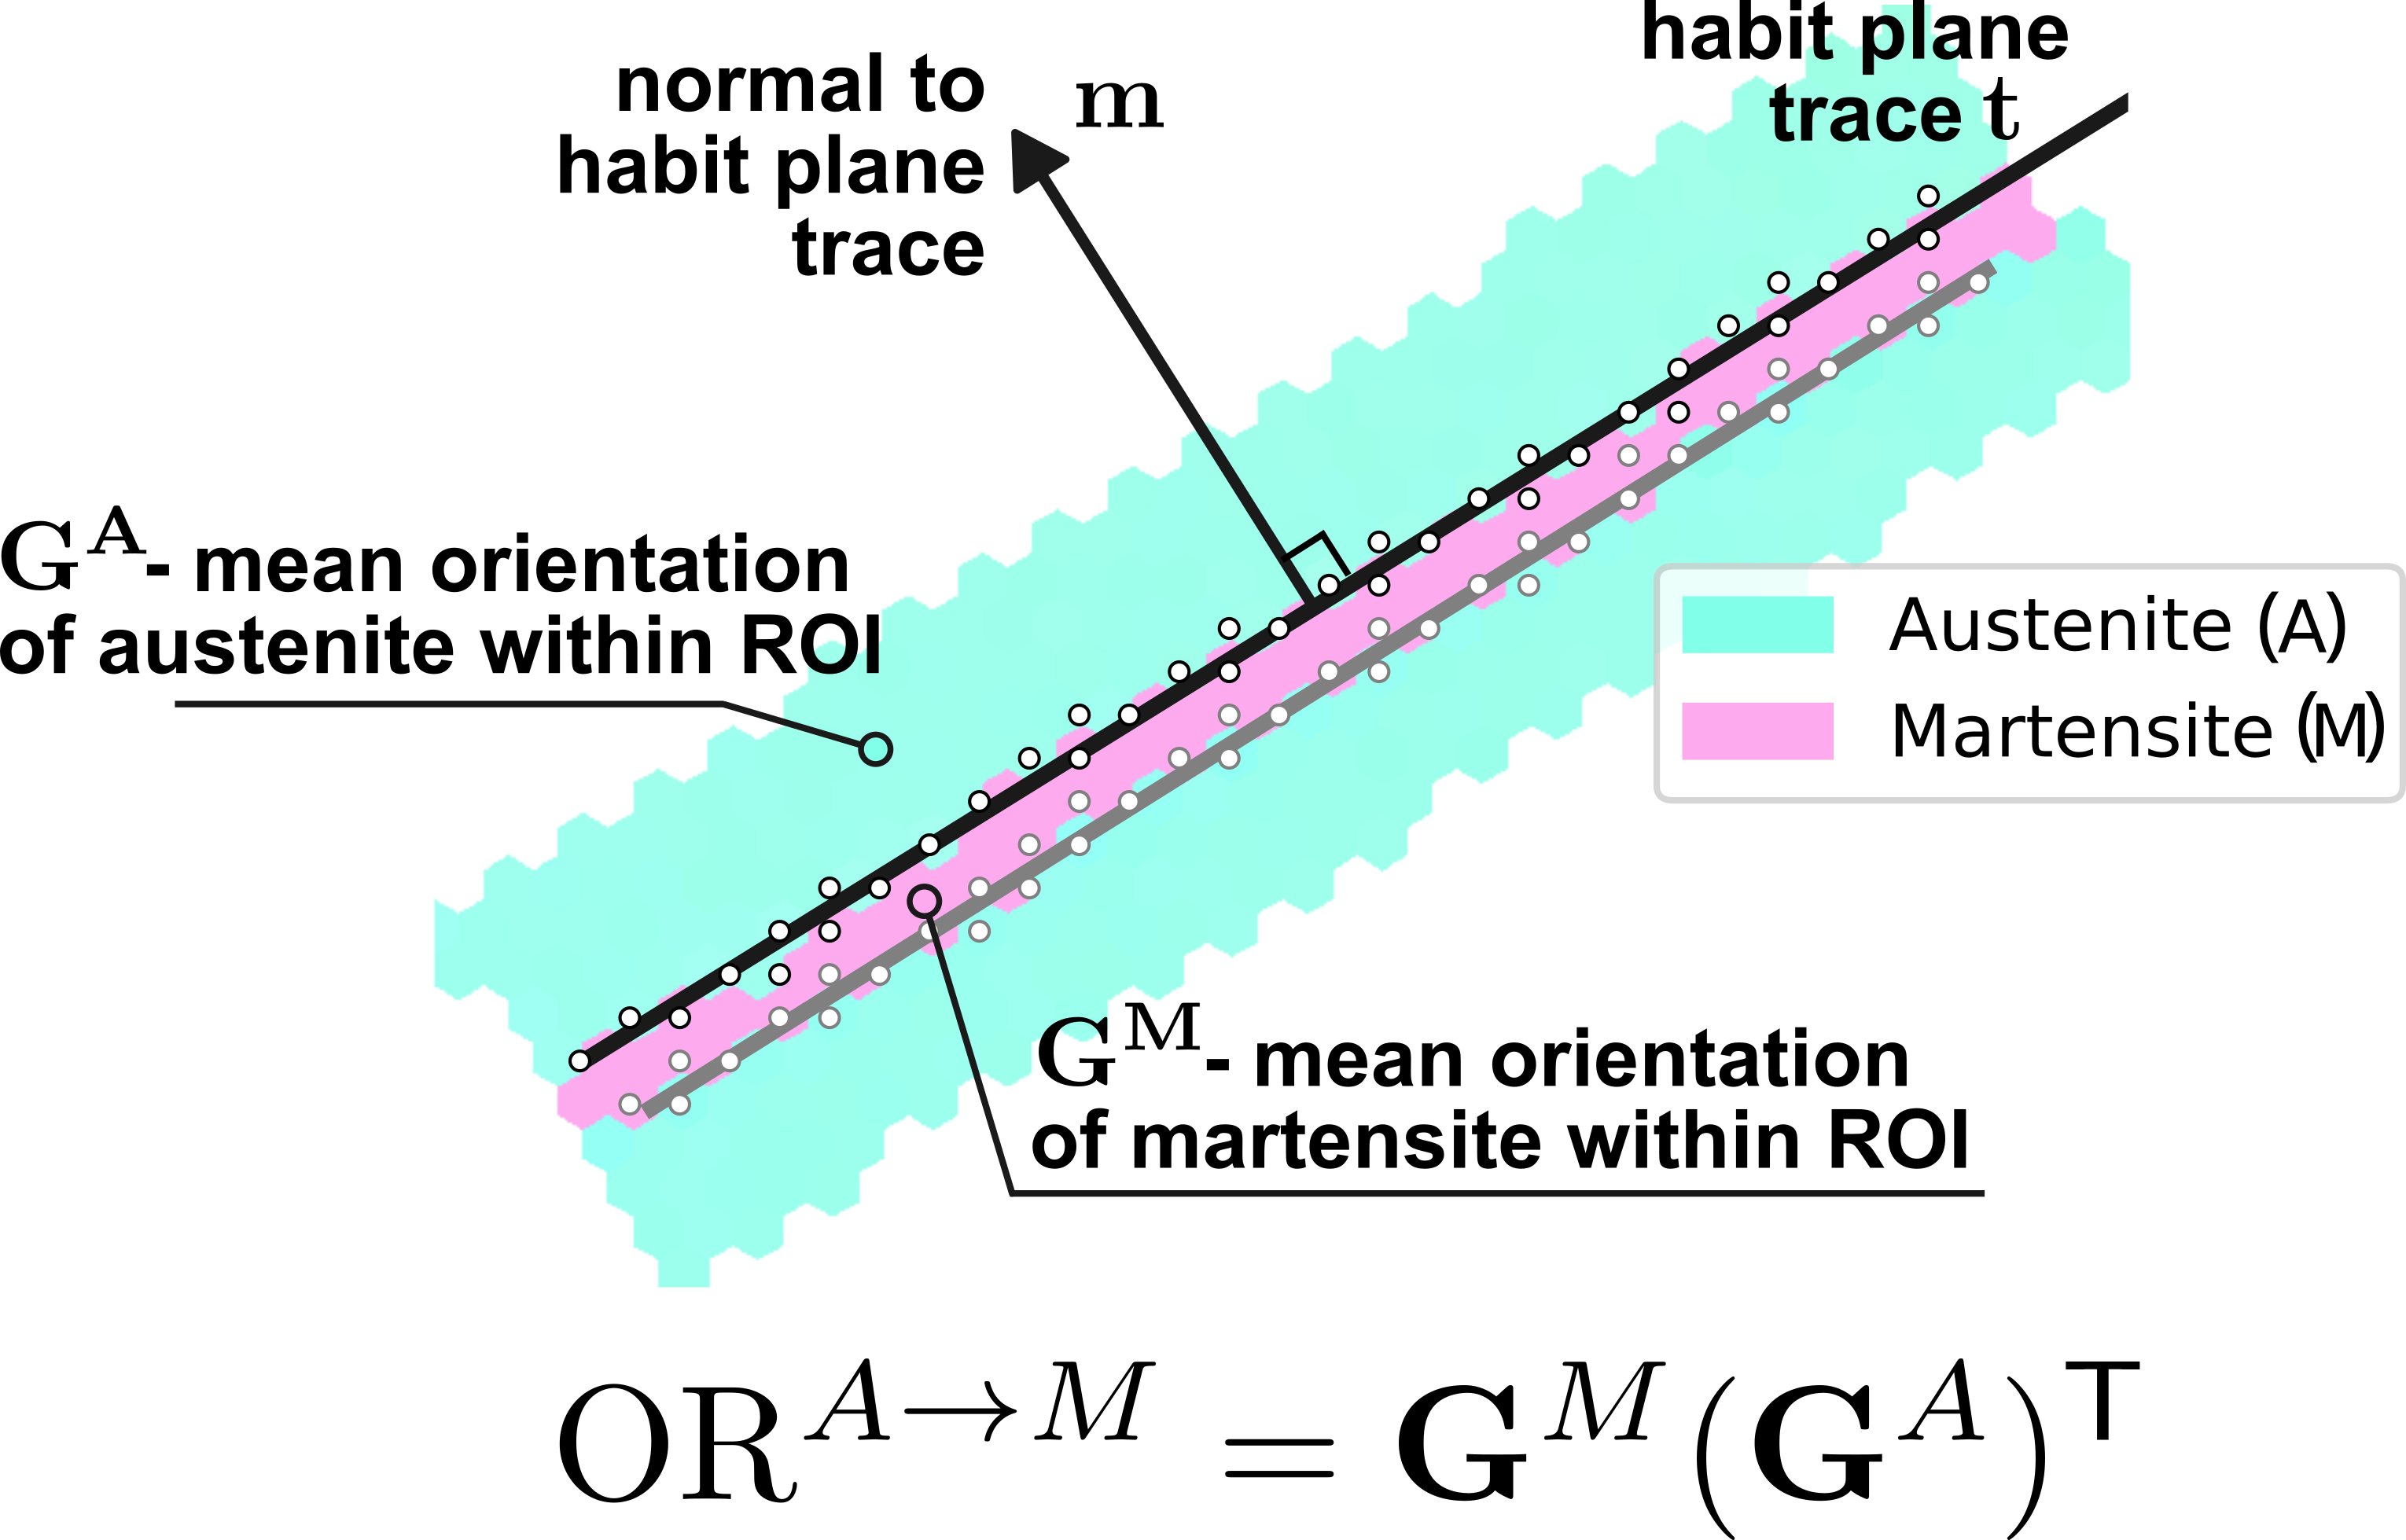
\includegraphics[width=0.92\linewidth]{./figs/fig_trace.png}
\caption{Identification of the orientation relationship and of the habit-plane trace on the ROI (view onto the scan surface). The interface boundary pixels $(X_i,Y_i)$ of the austenite and martensite sides are fitted by a straight line $y=kx+q$, giving the trace $\vc t$ and its in-plane normal $\vc m$, Eqs.~\eqref{eq:trace}--\eqref{eq:crystal_trace}. The mean side orientations $\mat G^{\mathrm A}$ and $\mat G^{\mathrm M}$ define the experimental orientation relationship $\mathrm{OR}^{A\to M}=\mat G^{\mathrm M}(\mat G^{\mathrm A})^{\mathsf T}$ (the symmetry-reduced average used in Eq.~\eqref{eq:expOR}). A single section reveals only the trace, so its normal is constrained merely to the plane perpendicular to $\vc t$, leaving one free rotation angle.}
\label{fig:trace}
\end{figure}

\begin{figure}[H]
\centering
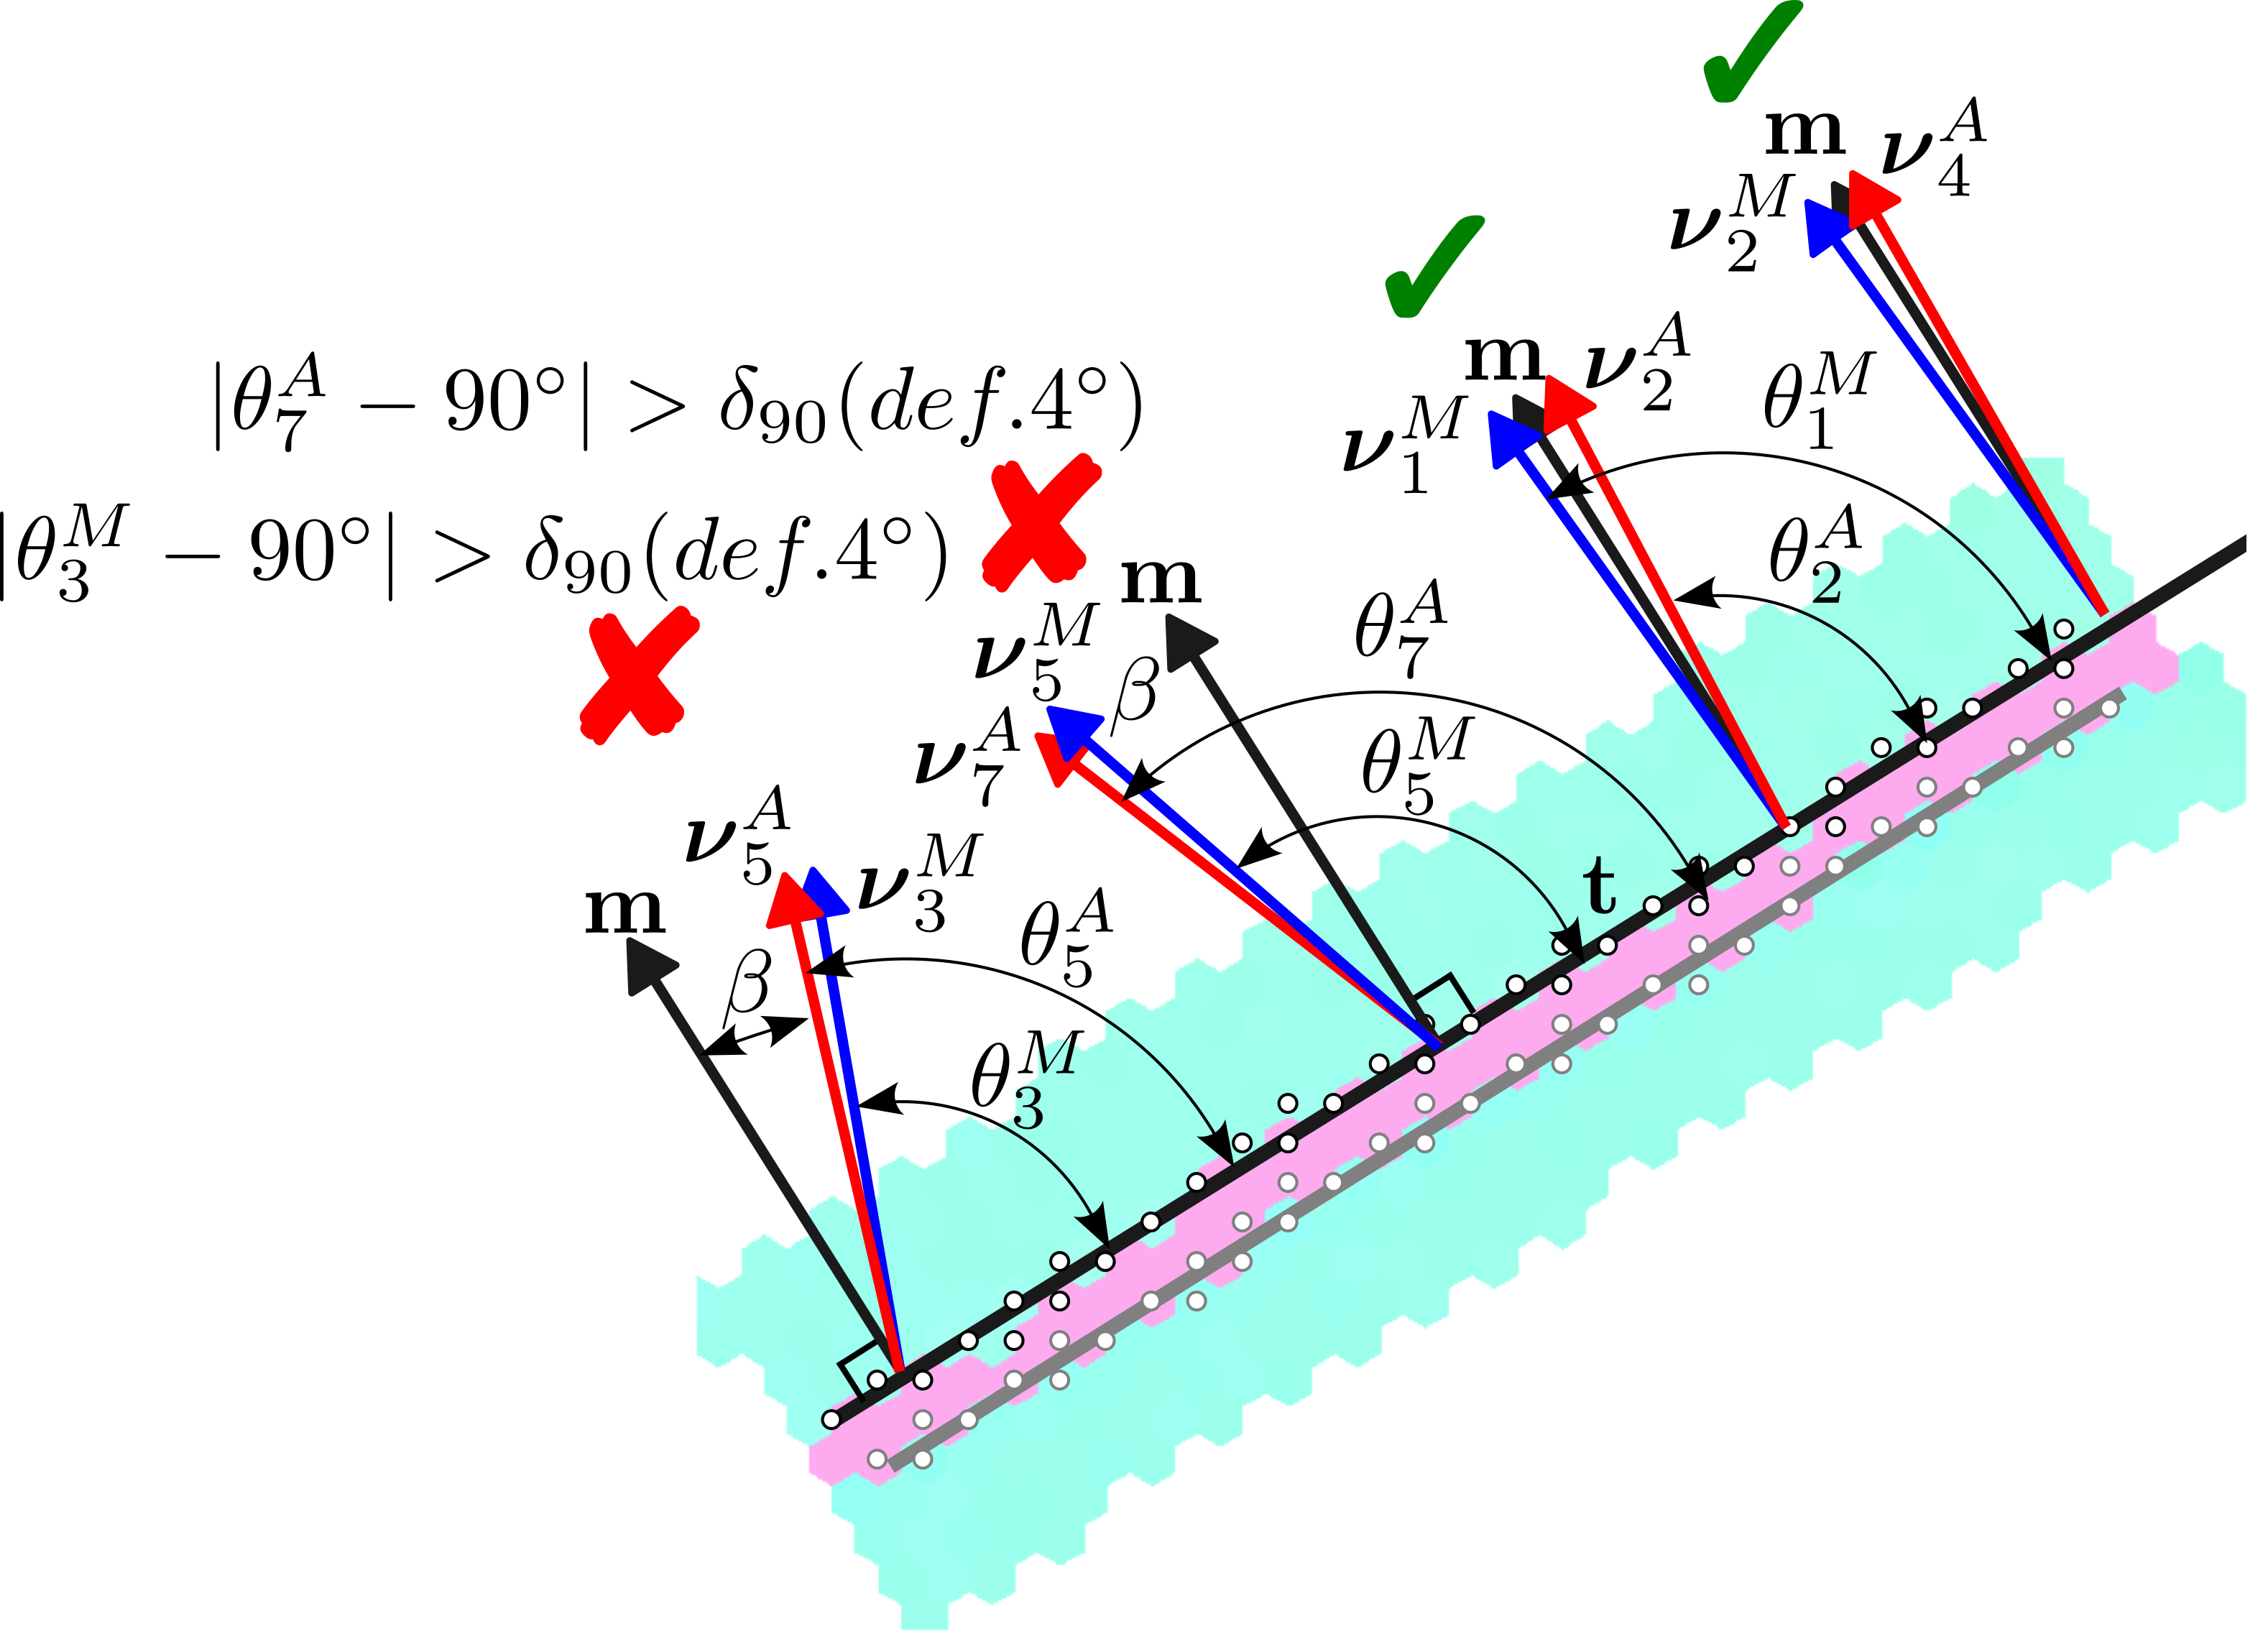
\includegraphics[width=0.92\linewidth]{./figs/fig_cand_par.png}
\caption{Trace-containment test of Eq.~\eqref{eq:accept}, viewed onto the scan surface (plane parallel to the trace). For each phase the candidate plane normals $\vc\nu^{\mathrm A}_i$ (red) and $\vc\nu^{\mathrm M}_j$ (blue) are projected at points along the trace. A candidate is accepted ($\checkmark$) when its normal is perpendicular to the trace within tolerance, $|\theta^{\varphi}-90^\circ|\le\delta_{90}$ (default $4^\circ$), with $\theta^{\varphi}=\arccos|\vc\nu^{\varphi}\cdot\vc t^{\,\varphi}|$, and rejected ($\times$) otherwise. The test is applied independently in austenite ($\varphi=\mathrm A$) and martensite ($\varphi=\mathrm M$).}
\label{fig:cand_par}
\end{figure}

\section{Experimental orientation relationship and variant identification}

Before the candidate planes of the two phases can be compared, the lattice-correspondence variant active at the analysed interface must be identified. From the averaged side orientations the experimental orientation relationship is formed for every proper symmetry operation $\mat S_i$ of the martensite,
\begin{equation}
\mat T^{\mathrm{exp}}_{\mathrm{AM},i}=\mat S_i\,\mat G^{\mathrm{M}}\,\mat G^{\mathrm{A}\,\mathsf T},
\label{eq:expOR}
\end{equation}
and compared with each theoretical variant $\mat T^{(v)}_{\mathrm{AM}}$ through the rotation $\mat D_{i v}=\mat T^{\mathrm{exp}}_{\mathrm{AM},i}\,\mat T^{(v)\,\mathsf T}_{\mathrm{AM}}$. Since the residual misorientation angle $\omega$ obeys $\cos\omega = \tfrac12\big(\trace \mat D_{iv}-1\big)$, the pair $(i^\ast,v^\ast)$ maximizing $\trace\mat D_{iv}$ identifies the closest variant (\texttt{getClosestOR}); $\omega(i^\ast,v^\ast)$ is reported as the OR misfit. For the selected variant the transformation strain along chosen sample directions $\vc l$ is evaluated from the deformation gradient,
\begin{equation}
\varepsilon(\vc l)=\sqrt{\vc l_{c}^{\mathsf T}\,\mat F^{(v^\ast)\,\mathsf T}_{\mathrm{AM}}\mat F^{(v^\ast)}_{\mathrm{AM}}\,\vc l_{c}}-1,
\qquad \vc l_c=\mat G^{\mathrm{A}}\vc l ,
\label{eq:strain}
\end{equation}
i.e.\ the relative length change of a material line along $\vc l$ caused by the transformation. The axis--angle representation of the average experimental OR, $\mat G^{\mathrm{M}}\mat G^{\mathrm{A}\,\mathsf T}$, is stored alongside.

\section{Cross-phase matching of candidates}

The habit plane is a physical interface shared by both lattices, so its normal must be the \emph{same vector in the sample frame} regardless of which phase is used to index it. The matching procedure \texttt{getHBmatches} therefore runs the candidate generation of the previous section independently for austenite and martensite, yielding indexed candidate sets $\{\vc h^{\mathrm A}_i\}$ and $\{\vc h^{\mathrm M}_j\}$, and tests every pair $(i,j)$ against
\begin{equation}
\Delta^{\mathrm{HP}}_{i,j}
=\arccos\big|\,\vc\nu^{\mathrm A,s}_{i}\cdot \vc\nu^{\mathrm M,s}_{j}\,\big|
\;\le\;\Delta_{\max},
\label{eq:hpmatch}
\end{equation}
where $\vc\nu^{\mathrm A,s}_{i}$ and $\vc\nu^{\mathrm M,s}_{j}$ are the sample-frame normals of austenite candidate $i$ and martensite candidate $j$ (Eq.~\eqref{eq:nu} mapped to the sample frame through $\mat G^{\varphi\,\mathsf T}$), and the threshold has default $\Delta_{\max}=2^\circ$ (\texttt{maxnormaldev}). Because each phase's candidate set already satisfies the per-phase trace-containment test of Eq.~\eqref{eq:accept}, every retained pair obeys $|\theta^{\mathrm A}_i-90^\circ|\le\delta_{90}$ and $|\theta^{\mathrm M}_j-90^\circ|\le\delta_{90}$ independently; the coincidence condition $\Delta^{\mathrm{HP}}_{i,j}\le\Delta_{\max}$ is the only criterion that couples the two phases.

\begin{figure}[H]
\centering
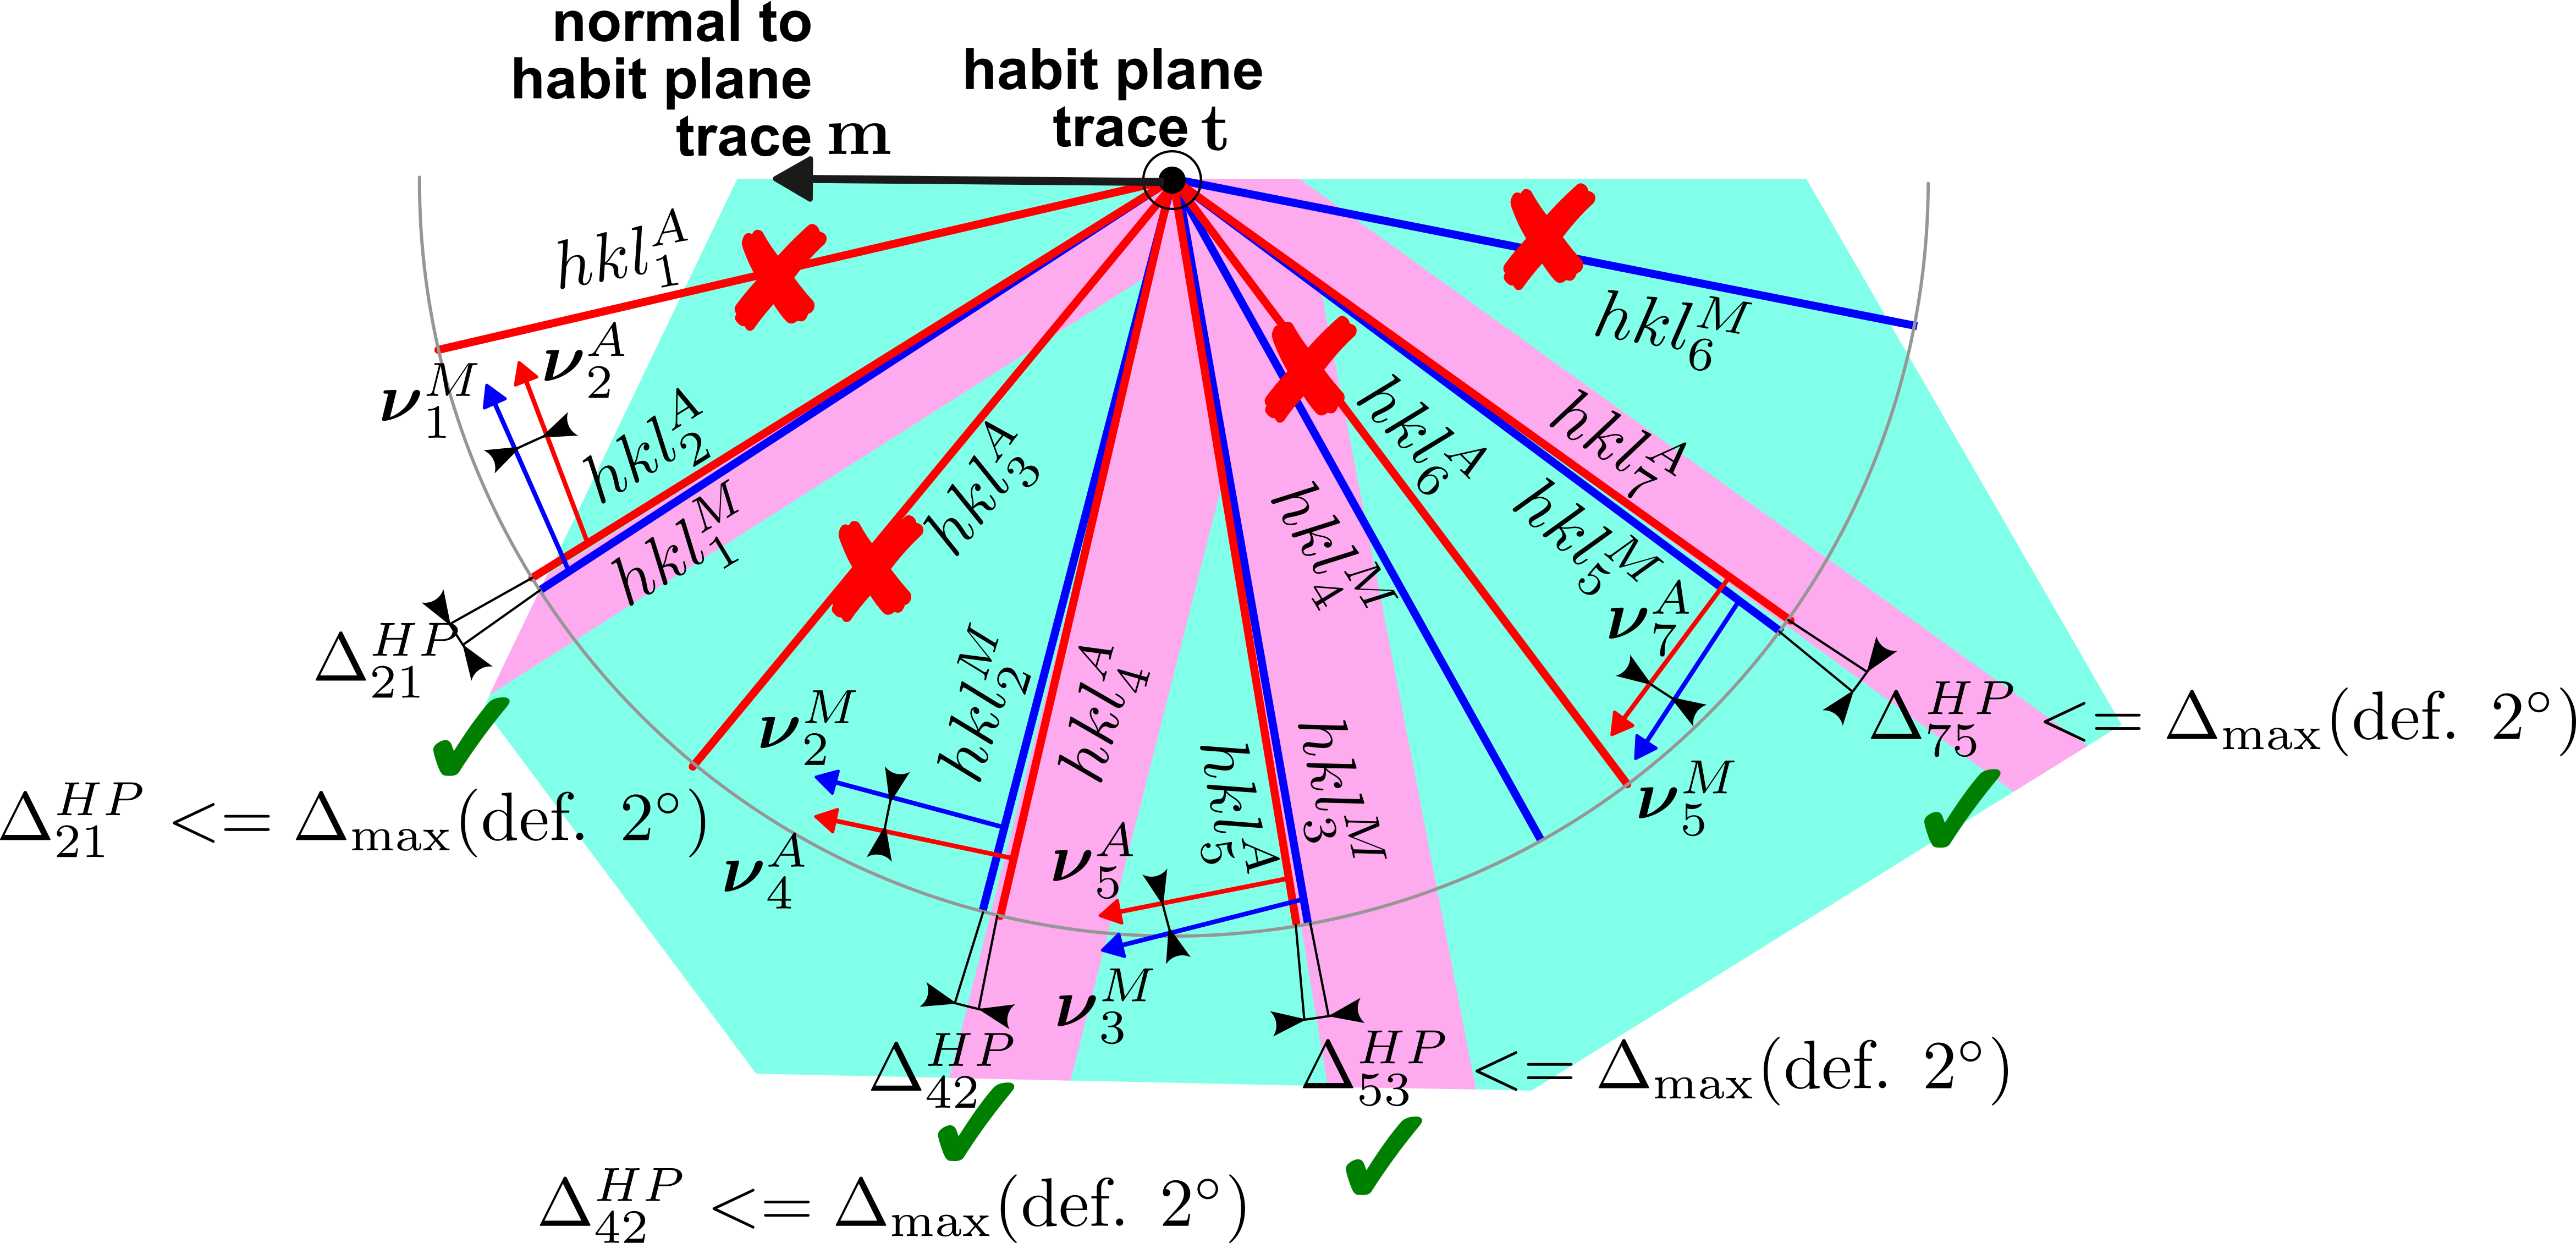
\includegraphics[width=0.86\linewidth]{./figs/fig_cand_perp.png}
\caption{Cross-phase matching in the fictitious cross-section perpendicular to the trace, in which the trace $\vc t$ points out of the plane and every admissible candidate plane appears edge-on as a line through the centre. Low-index candidates of austenite (red, planes $hkl^{\mathrm A}_i$ with normals $\vc\nu^{\mathrm A}_i$) and martensite (blue, planes $hkl^{\mathrm M}_j$ with normals $\vc\nu^{\mathrm M}_j$) are drawn at their respective angles. A pair $(i,j)$ is accepted ($\checkmark$) when the two indexed normals coincide in the sample frame within $\Delta^{\mathrm{HP}}_{i,j}\le\Delta_{\max}$ (default $2^\circ$), Eq.~\eqref{eq:hpmatch}; candidates of one phase without a matching partner in the other ($\times$) are discarded.}
\label{fig:cand_perp}
\end{figure}

For each surviving pair, corresponding \emph{in-plane lattice directions} are sought. Within each phase, the same rotational sampling of Eq.~\eqref{eq:family} is reused with the roles exchanged: the rotation axis is now the candidate plane normal $\vc\nu^{\varphi}(\vc h^{\varphi})$, the direct structure matrices $\mat L^{\varphi}$, $(\mat L^{\varphi})^{-1}$ replace the reciprocal ones, and the perpendicularity tolerance is set to zero, which yields the low-index lattice directions $\vc u^{\varphi}$ lying exactly in the candidate plane ($\vc u^{\varphi}\perp\vc\nu^{\varphi}$). Direction pairs $(\vc u^{\mathrm A},\vc u^{\mathrm M})$ are accepted when their sample-frame misalignment is below $\delta_d=2^\circ$ (\texttt{maxdirdev}), keeping for each austenite direction only the best-matching martensite partner. A plane pair is retained only if at least one corresponding direction pair exists.

Finally, the retained pair is tested for consistency with the lattice correspondence of the identified variant. With the martensite symmetry operation $\mat S_{i^\ast}$ from Eq.~\eqref{eq:expOR}, the correspondence predicts
\begin{equation}
\vc h^{\mathrm M}_{\mathrm{pred}}=\operatorname{red}\big(\mat S_{i^\ast}\,\mat C_p^{(v^\ast)}\,\vc h^{\mathrm A}\big),
\qquad
\vc u^{\mathrm M}_{\mathrm{pred}}=\operatorname{red}\big(\mat S_{i^\ast}\,\mat C_d^{(v^\ast)}\,\vc u^{\mathrm A}\big),
\label{eq:corresp}
\end{equation}
and the boolean flag \texttt{fitcorresp} records whether $\vc h^{\mathrm M}_{\mathrm{pred}}=\pm\vc h^{\mathrm M}$ and $\vc u^{\mathrm M}_{\mathrm{pred}}=\pm\vc u^{\mathrm M}$ hold for the plane and for all matched directions. This distinguishes candidate pairs that merely happen to be parallel in space from pairs that are crystallographically the same plane and directions inherited through the transformation.

\section{Scoring and ranking}

Each matched candidate pair $(i,j)$ receives the score
\begin{equation}
S_{i,j} \;=\; \frac{\sum_k |h^{\mathrm A}_{i,k}| + \sum_k |h^{\mathrm M}_{j,k}|}{N_d}
\;+\;
\bar\Delta_{i,j},
\qquad
\bar\Delta_{i,j}=\frac{1}{N_d+3}\Big(\sum_{l=1}^{N_d}\delta_l
+\big|\theta^{\mathrm A}_i-90^\circ\big|
+\big|\theta^{\mathrm M}_j-90^\circ\big|
+\Delta^{\mathrm{HP}}_{i,j}\Big),
\label{eq:score}
\end{equation}
where $i$ and $j$ index the austenite and martensite candidate of the pair, $h^{\mathrm A}_{i,k}$ ($k=1,2,3$) are the Miller components of austenite candidate $i$ (and likewise $h^{\mathrm M}_{j,k}$), $N_d$ is the number of matched direction pairs, $\delta_l$ their misalignments, $\theta^{\mathrm A}_i$ and $\theta^{\mathrm M}_j$ the trace-containment angles of Eq.~\eqref{eq:accept} and $\Delta^{\mathrm{HP}}_{i,j}$ the normal misalignment of Eq.~\eqref{eq:hpmatch}. Lower scores are better: the first term penalizes high Miller indices and rewards a rich set of corresponding directions, the second penalizes geometric misfit. All result arrays are sorted by ascending $S_{i,j}$, and \texttt{printHBmatches} reports, per candidate, the indexed plane in both phases with their families, the misalignments, the score, the correspondence-consistency flag, and the transformation strain of the closest variant from Eq.~\eqref{eq:strain}.

\section{Variant-resolved propagation between phases}

As an alternative to the symmetric matching of both phases, \texttt{getHB} generates candidates in a single seed phase (by default austenite, \texttt{phase4HPguess}) using Eq.~\eqref{eq:family}--\eqref{eq:accept} and then propagates each candidate into the second phase through the correspondence matrices (\texttt{getCorrespNormals}),
\begin{equation}
\vc h^{\mathrm M}=\mat C_p^{(v)}\,\vc h^{\mathrm A},
\qquad
\vc\nu^{\mathrm M}=\frac{\mat L_{r}^{\mathrm M}\,\vc h^{\mathrm M}}{\lVert \mat L_{r}^{\mathrm M}\,\vc h^{\mathrm M}\rVert},
\label{eq:propagate}
\end{equation}
evaluated both for the closest variant $v^\ast$ and for all variants. The propagated normal is scored by its trace-containment angle $\arccos|\vc\nu^{\mathrm M}\cdot\vc t^{\,\mathrm M}|$ in the second phase, and plane/direction candidate lists are sorted by the combined deviation of both phases from the ideal $90^\circ$. The same machinery applied with the direct lattice ($\mat L^{\varphi}$, $\mat C_d$) yields in-plane direction candidates.

\section{Workflow summary and parameters}

For a chosen parent--child pair and semi-ROI, \texttt{singleHP} executes the chain \texttt{getOri} (averaged side orientations, pole figures, experimental OR, closest variant and transformation strains), \texttt{getInterface} (trace fit, Eqs.~\eqref{eq:trace}--\eqref{eq:crystal_trace}), \texttt{getHBmatches} (candidate generation, cross-phase matching, correspondence check and scoring, Eqs.~\eqref{eq:family}--\eqref{eq:score}) and optionally \texttt{printHBmatches}. Semi-ROIs without a parent side (\texttt{no\_parent\_side}) are skipped. Table~\ref{tab:params} lists the user-adjustable tolerances.

\begin{table}[ht]
\centering
\caption{Tolerances of \texttt{EbsdHPAnalyzer} (constructor arguments) and their role.}
\label{tab:params}
\begin{tabular}{lcl}
\toprule
Parameter & Default & Meaning \\
\midrule
\texttt{maxmillerindex} ($h_{\max}$) & 4 & Largest admissible Miller index of a candidate plane/direction \\
\texttt{maxdevfrom90deg} ($\delta_{90}$) & $4^\circ$ & Tolerance on trace containment, Eq.~\eqref{eq:accept} \\
\texttt{maxnormaldev} ($\Delta_{\max}$) & $2^\circ$ & Tolerance on cross-phase normal coincidence, Eq.~\eqref{eq:hpmatch} \\
\texttt{maxdirdev} ($\delta_d$) & $2^\circ$ & Tolerance on cross-phase in-plane direction coincidence \\
\bottomrule
\end{tabular}
\end{table}

\section{Remarks and limitations}

A single planar trace cannot determine a plane uniquely; the method compensates by combining four independent constraints: trace containment in \emph{both} crystal frames, spatial coincidence of the indexed normals, existence of matching low-index in-plane directions, and agreement with the lattice correspondence of the variant deduced from the measured orientation relationship. The accuracy is limited by the linearity of the boundary (curved or stepped interfaces degrade the least-squares trace fit), by the orientation noise entering the averaged matrices $\mat G^{\varphi}$, and by the discretization of the rotational sampling ($0.5^\circ$). The angular tolerances should be kept consistent with the typical EBSD orientation precision ($\sim$0.5--2$^\circ$); enlarging $h_{\max}$ rapidly increases the number of geometrically admissible but physically meaningless high-index candidates, which the low-index term in the score of Eq.~\eqref{eq:score} suppresses only partially. Where a lamella offers two well-separated semi-ROIs, running the analysis on both and comparing the ranked candidates provides an internal consistency check; agreement of the top-ranked plane across semi-ROIs and across lamellae of the same variant is the strongest practical validation of the estimated habit plane.

\end{document}
